% =========================================================================== %

\begin{frame}[t,plain]
\titlepage
\end{frame}

% =========================================================================== %

\begin{frame}{Paths}
%
\begin{columns}
\column{.6\linewidth}
\begin{center}
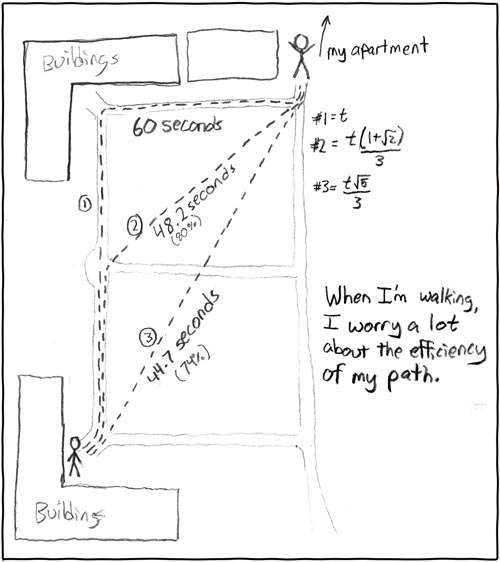
\includegraphics[width=0.6\linewidth]{./gfx/04-xkcd-paths}\\
\end{center}
%
\column{.2\linewidth}
\small
	\emph{It's true, I think about this all the time.}

	\vspace{6pt}
	\url{https://xkcd.com/85/}
\end{columns}
%
\end{frame}

% =========================================================================== %

\begin{frame}{Scope for Today}
%
\begin{itemize}
\item Numerical integration to find trajectories
	\begin{itemize}
	\item \texttt{scipy.integrate.solve\_ivp}
	\item Runge-Kutta-Integrator
	\item Leapfrog-Integrator
	\end{itemize}
\item Differential equations as eigenvalue problems
	\begin{itemize}
	\item \texttt{np.linalg.eig} and \texttt{eigh}
	\item Sparse matrices
	\item Numerical stability
	\end{itemize}
\end{itemize}
%
\end{frame}

% =========================================================================== %

\begin{frame}{Solving Initial Value Problems}
%
\begin{itemize}
\item Scenario
	\begin{itemize}
	\item Given: Function $f: \dv{t} y(t) = f(t, y)$
	\item Given: $y_0 = y(t_0)$
	\item Known: $y \in \mathbb{C}^{D}$
	\item Wanted: values $y_i = y(t_i)$ for arbitrary $t_i \in [t_0, t_N]$
	\end{itemize}
\item Solution
	\begin{itemize}
	\item \texttt{scipy.integrate.solve\_ivp}
	\item Most simple form: \texttt{result = solve\_ivp(f, [t\_0, t\_N], [y\_0])}
	\item \texttt{result} is of type \texttt{scipy.integrate.\_ivp.ivp.OdeResult}, which has attributes \texttt{t} and \texttt{y}
	\item \texttt{result.t} contains the $t_i$ as a Numpy array
	\item \texttt{result.y} contains the $y_i$ as a Numpy array
	\end{itemize}
\end{itemize}
%
\end{frame}

% =========================================================================== %

\begin{frame}[fragile]{A More Detailled Look at The Solver: The function \texttt{f}}
%
\begin{itemize}
\item Callable
	\begin{itemize}
	\item May be a regular Python function (\inPy{def f(t, y): ...})
	\item May be a Lambda (\inPy{f = lambda t, y: ...})
	\item May be a class instance with a dunder call (\inPy{def __call__(self, t, y): ...})
	\end{itemize}
\item Parameters
	\begin{itemize}
	\item MUST accept parameters \texttt{t, y} in that oder
	\item May accept more parameters (we'll see later on)
	\item \texttt{t} -- time-like variable, \enquote{external} to the system
	\item \texttt{y} -- state-like variable, \enquote{the system at time \texttt{t}}
	\end{itemize}
\item Return Value
	\begin{itemize}
	\item $y'(t)$
	\item As a scalar if $y(t)$ is a scalar function
	\item As an iterable (\zB \inPy{list}, \inPy{tuple} or \inPy{np.array}), if $y(t)$ is a vector valued function
	\end{itemize}
\end{itemize}
%
\end{frame}

% =========================================================================== %